\pagebreak
\chapter{Implementation}
\section{Tree Creation}
To create a tree from a graph there are different approaches to describe the angles as mentioned in section \ref{sec:tree_creation_angle}. For the implementation in CPlan the used approach was the method two where straight forward is described with +180 degrees. If only positive angles exist the absolute value of a given graph would also generate a correct result.

Because a tree can not fully represent a graph, many points exist multiple times in the resulting tree. To recreate a graph, junctions should be added where streets intersect without junctions. And the resulting graph should be snapped where points are at the same position. Additionally the existing multiple points in the graph should be removed.

This forward an backward transformation between a graph and a tree allows to run a genetic algorithm like mutation or crossover on a tree and display the result as graph. These genetic algorithm were already implemented by the \acrlong{iA}.

\pagebreak
\section{K-Means}
To separate street networks the centroid based clustering algorithm K-Mean can be used. The added implementation in CPlan \citep{cPlan:2015} is based on the approach described in section \ref{sec:K-Means}. Some libraries used by CPlan provide the K-Means clustering already but this approach would not allow a visualisation of the progress and a speed up by parallelisation.

\subsection{Connected Cluster Implementation} \label{sec:K-Means_shortest_path_impl}
As described in section \ref{sec:connected_cluster_approach} the edge based distances can be calculated with a \gls{APSP} algorithm. Based on these distances the cluster points are then assigned. The result is a connected graph. This means every vertex can be reached from every other vertex within a cluster. In the generated figure \ref{fig:Kmeansshortestp} the artefacts described in \ref{sec:K-Means_shortest_path} are removed.

Additional calculation time is needed for the shortest path algorithm. The differences can be compared in the section Measurements \ref{sec:measurements-speed}.

\subsection{Speed Optimization}
The ETH-Zurich provided the following networks: Bad Berka (552 nodes, 626 edges), Weimar (2012 nodes, 2646 edges) and Zurich (27446 nodes, 35121 edges). The street network of Zurich has 13 times more edges than Weimar, which resulted in long processing times. A speed improvement was achieved by running the K-Means iterations paralllised. Every iteration can be executed free of side effects. The measurements and comparisons of the results are provided in the following section \ref{sec:measurements-speed}.

Additional acceleration would be possible by using K-Means++ \ref{sec:k-means++} or a K-D tree \ref{sec:k-means_KD-tree}.

\pagebreak
\section{WPGMA / UPGMA}
\subsection{Memory Usage Optimisations} \label{sec:memory_usage}
In section \ref{sec:concept_memory_usage} of the concept chapter, the problem of high memory usage is discussed. In this section three applied optimisations are explained in more detail.

The easiest optimisation is to convert all distances to a single-precision floating-point format. The loss of precision is not affecting the result, as mostly only the $<$ and $>$ relations of the different distances are important.

A second optimisation that can be applied is, to remove redundant information. When storing the full matrix of all distances, most values are stored twice. The matrix is mirrored along the diagonal, because the used street networks are undirected graphs. So the memory usage can almost be cut in half if those duplicates are not stored. This improvement is visualised in figure \ref{fig:memory_usage_01}.

The third and last applied optimisation was to change the way, how cluster distances are stored if the reduction formula \acrshort{UPGMA} or \acrshort{WPGMA} is used. Each time, when two clusters are combined, the distances of the new formed cluster to every other cluster are calculated. This combination step is done using the distances stored for the two old clusters. Afterwards the distances which were stored for the old clusters are no longer used. To reduce the memory usage, the distances of the new cluster can therefore be stored at the location where the distances of one of the old clusters were stored. Figure \ref{fig:memory_usage_02} visualises this optimisation.

When applying those memory usage optimisations, $\frac{1}{2}n(n+1)$ single-precision floating point numbers have to be stored. The memory complexity still lies in $O(n^2)$, but the improvements allow most modern computers to analyse medium to big sized street networks. As an example: For the used environment the memory usage would amount to about 1.36 Gigabyte for the street network of Zurich.

\begin{figure}
    \centering
    \begin{subfigure}[b]{\textwidth}
        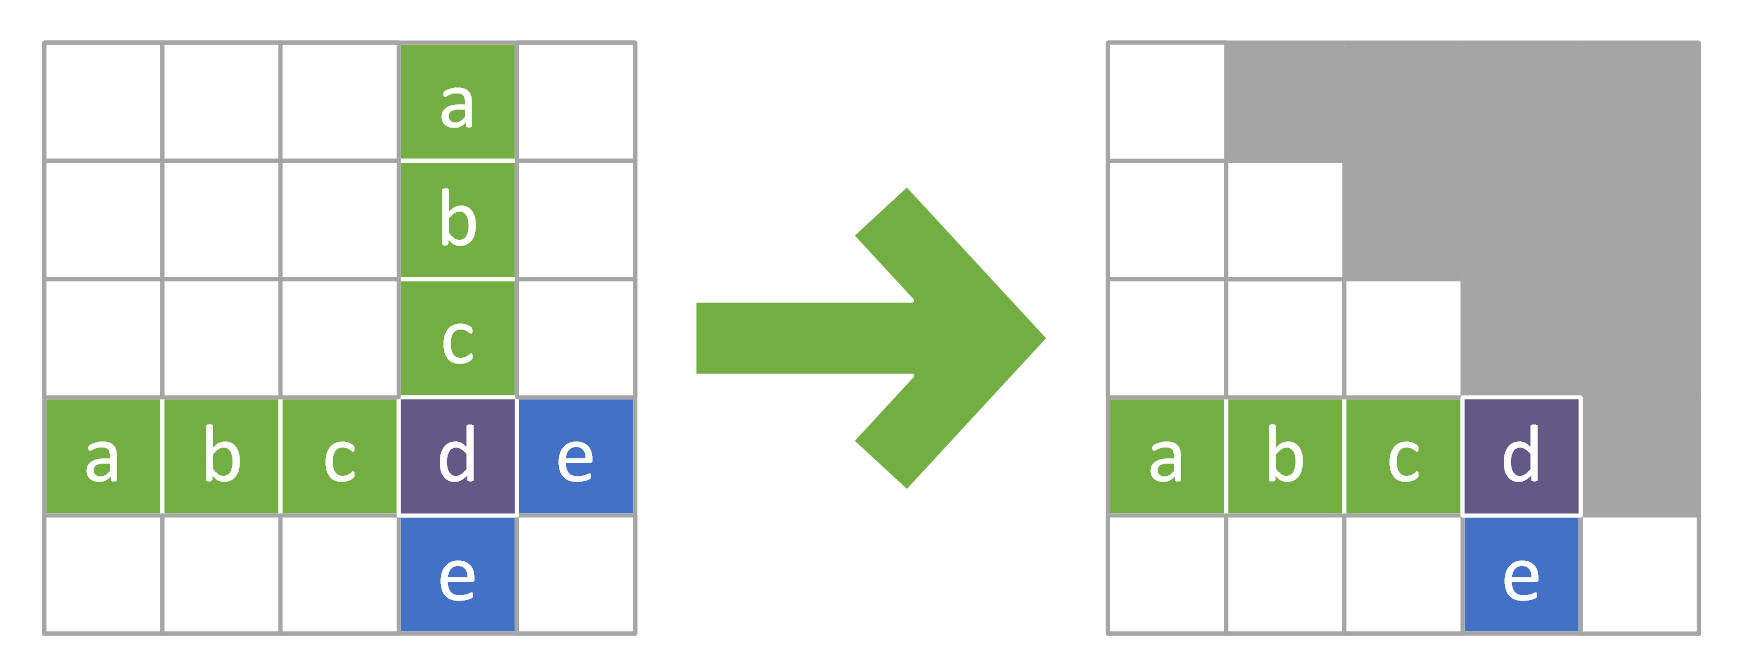
\includegraphics[width=\linewidth]{memoryusage01.png}
        \caption{Optimisation of memory usage by not storing redundant information. On the left hand side is the full distance matrix, on the right hand side is the same matrix without the duplicate entries.}
        \label{fig:memory_usage_01}
    \end{subfigure}
    \par\medskip
    \begin{subfigure}[b]{\textwidth}
        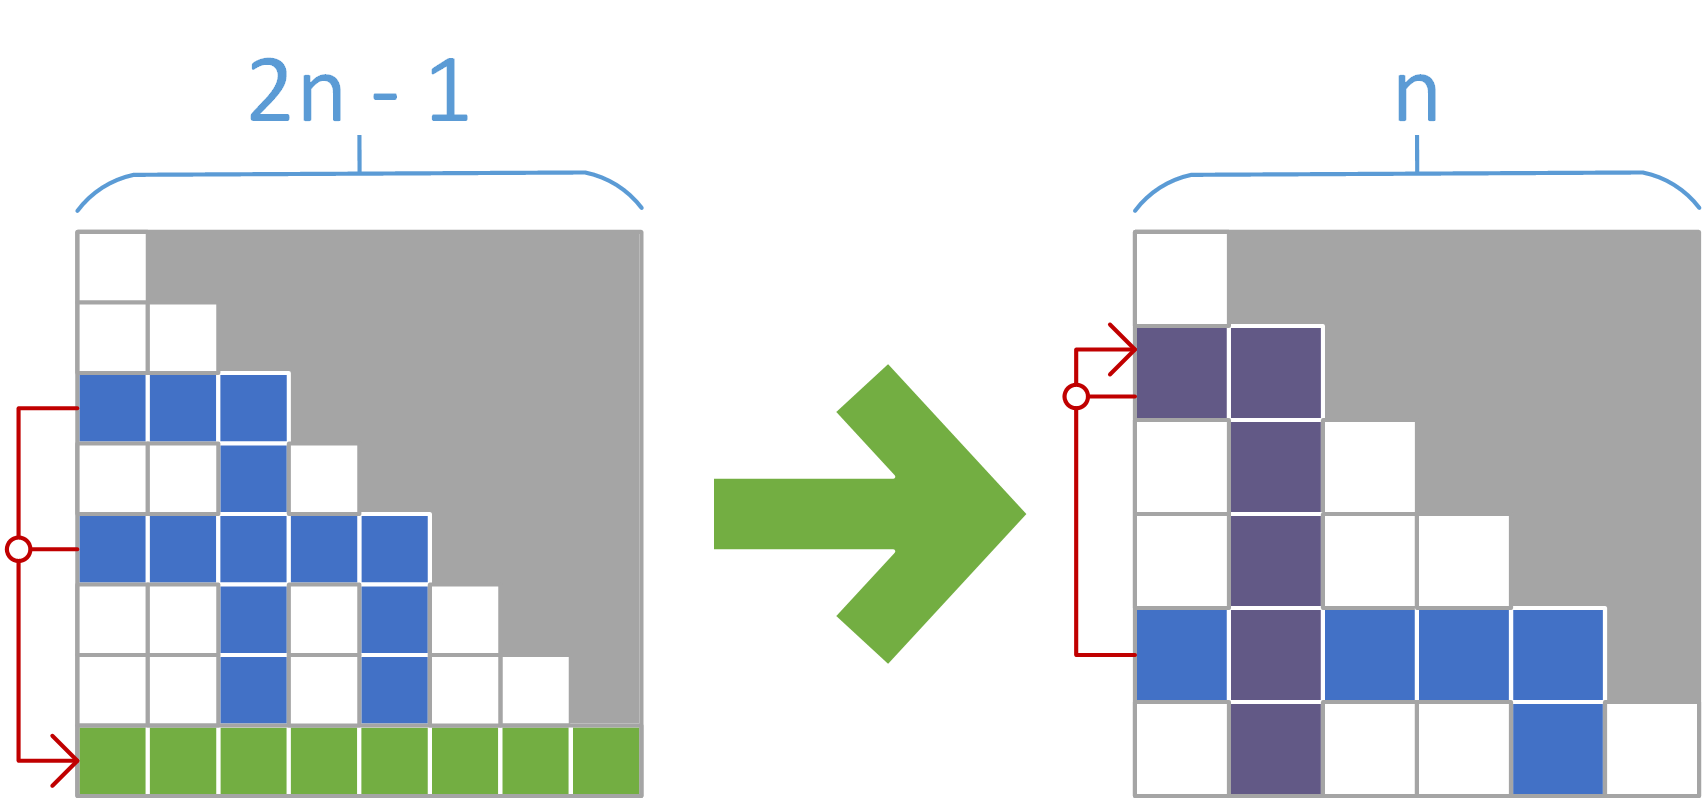
\includegraphics[width=\linewidth]{memoryusage02.png}
        \caption{Optimisation of memory usage by changing the cluster combination behaviour. On the left hand side the blue distances belonging to the old clusters are combined and stored in a new row (of green distances) belonging to the new formed cluster. The right hand side is similar, but the distances of the old clusters (blue and violet) are combined and stored at the location of one of the old clusters (violet). After the combination, the violet distances belong to the new formed cluster.}
        \label{fig:memory_usage_02}
    \end{subfigure}
    \caption{Visualised memory usage optimisations}
\end{figure}

\pagebreak
\subsection{Output Modification} \label{sec:outout_modification}
As shown in section \ref{sec:concept_cluster_sizes} there exist some cases, where hierarchical clustering has an output of clusters with highly varying size if standard splitting order is used. (Size meaning the vertex / street junction count in this context.)

Depending on the requirements this is the desired result, as it is the optimal solution of the algorithm using the given distances. In other cases it is more important, that the created clusters are roughly the same size, than it is to abide the mathematically optimal solution.

To create relatively equally sized clusters from the resulted hierarchy of a hierarchical cluster algorithm the following approach was taken. Instead of splitting the hierarchy into clusters exactly in the order in which the hierarchy was created, the order is changed. By always splitting the biggest cluster (cluster with the most nodes), a result with much more equally sized clusters will be created. A clustering with such modified sizes is shown in figure \ref{fig:modified_cluster_size}.

\begin{figure}
    \centering
    \begin{subfigure}[b]{0.49\textwidth}
        \begin{mdframed}[style=mdthight, userdefinedwidth=0.9\linewidth]
            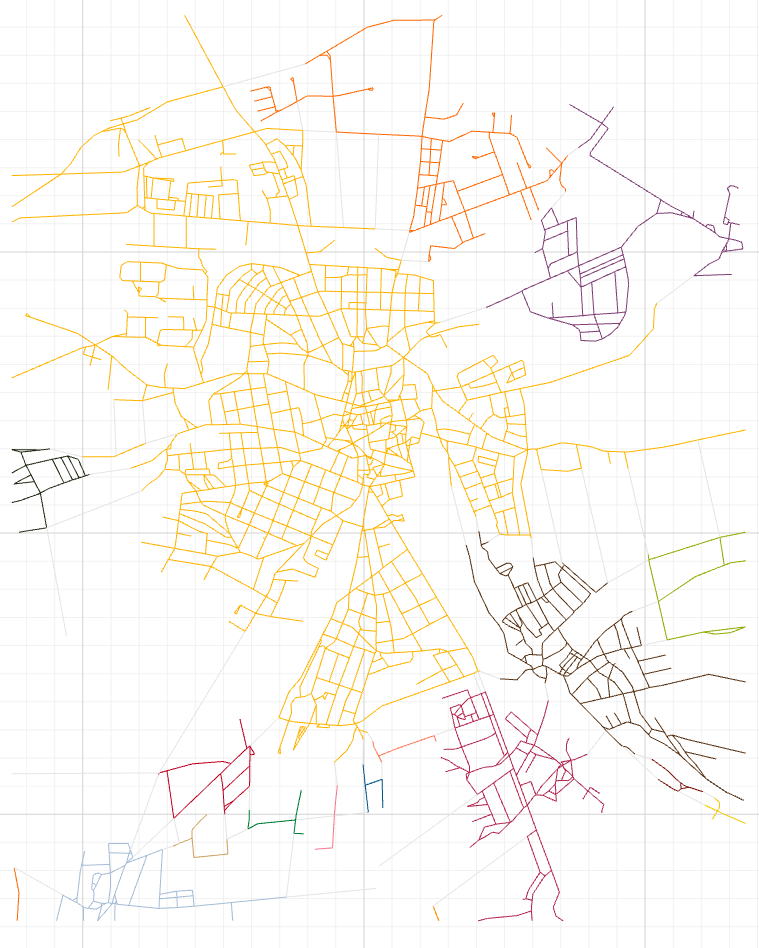
\includegraphics[width=\linewidth]{unmodified_cluster_size.png}
        \end{mdframed}
        \caption{Clusters with original size}
        \label{fig:unmodified_cluster_size}
    \end{subfigure}
    \begin{subfigure}[b]{0.49\textwidth}
        \begin{mdframed}[style=mdthight, userdefinedwidth=0.9\linewidth]
            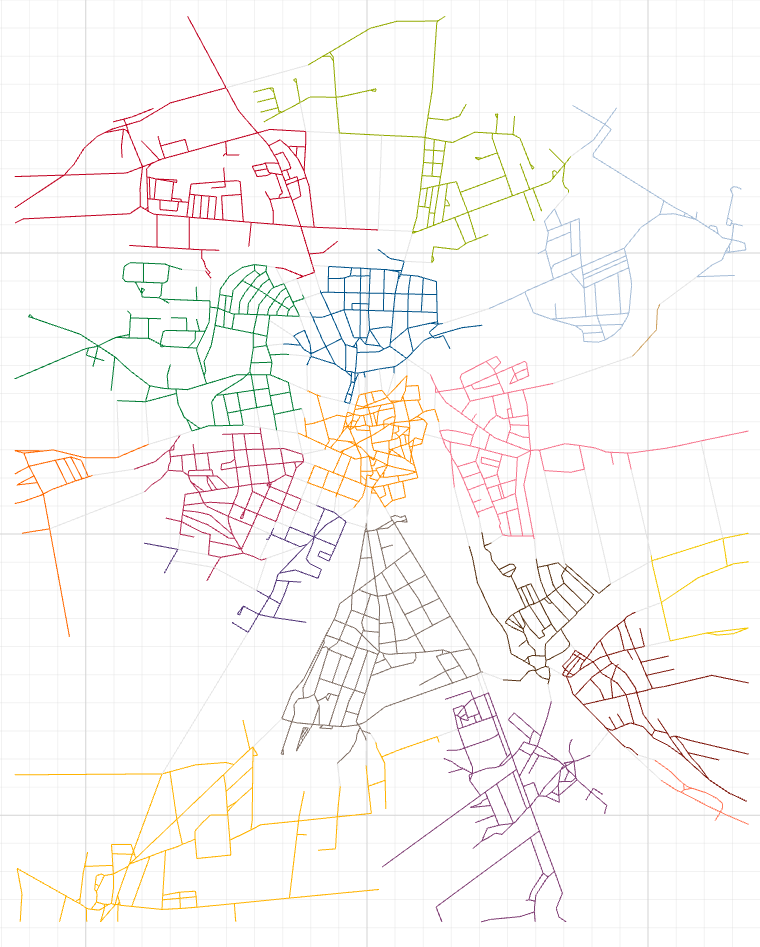
\includegraphics[width=\linewidth]{modified_cluster_size.png}
        \end{mdframed}
        \caption{Clusters with modified size}
        \label{fig:modified_cluster_size}
    \end{subfigure}
    \caption{Clustered street network of Weimar without \ref{fig:unmodified_cluster_size} or with \ref{fig:modified_cluster_size} cluster size modification. (Cluster count = 18, Reduction Formula = \acrshort{UPGMA})}
\end{figure}

\pagebreak
\section{Normalising Street Networks}
While testing clustering algorithms on the street network of Zurich one rough spot of this network was found: Not all streets, which lead to a junction are connected to it. As shown in figure \ref{fig:zuerich_error} floating streets exist (highlighted in purple). No end of any of these highlighted streets is connected to the rest of the street network.

To handle those floating streets a network normalisation method was developed. The normalisation snaps (unites) all junctions and street end points, which are positioned close together, into one common junction. The result of this normalisation is shown in figure \ref{fig:zuerich_fixed}.

\begin{figure}
    \centering
    \begin{subfigure}[b]{0.8\textwidth}
        \begin{mdframed}[style=mdthight]
            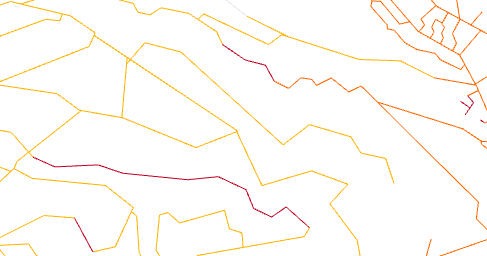
\includegraphics[width=\linewidth]{zuerich_street_error_cropped.png}
        \end{mdframed}
        \caption{Floating streets in the street network of Zurich}
        \label{fig:zuerich_error}
    \end{subfigure}
    \par\medskip
    \begin{subfigure}[b]{0.8\textwidth}
        \begin{mdframed}[style=mdthight]
            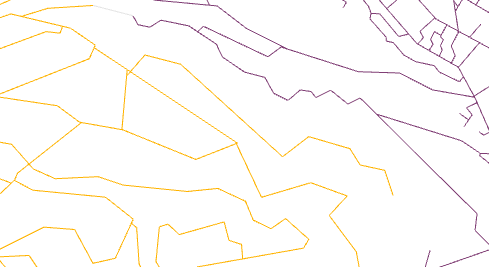
\includegraphics[width=\linewidth]{zuerich_street_fixed_cropped.png}
        \end{mdframed}
        \caption{Normalised street network of Zurich}
        \label{fig:zuerich_fixed}
    \end{subfigure}
    \caption{Street network of Zurich without (\ref{fig:zuerich_error}) and with (\ref{fig:zuerich_fixed}) normalisation}
\end{figure}

\section{Cluster colouring}
To visualize the clustering of a street network in this thesis, clusters are marked with different colours. This section describes the details of this cluster colouring.

The result of each clustering algorithm, which was implemented in this thesis, represents a cluster as set of vertices. Each of these vertices is a junction in the street network. The visualisation only draws streets but not the junctions, as the intersection of streets are intuitively seen as junctions. To colour the different clusters the following approach was taken:

\begin{itemize}
    \item Streets which connect two vertices that are part of the same cluster are coloured with that clusters colour.
    \item Streets which connect vertices of two distinct clusters are coloured grey.
\end{itemize}

There are papers which discuss how colours can be transformed to a perceptually uniform space, where the computation of $n$ colours with maximal distances (for the human eye) is possible \cite{colors:2006}.

In this thesis a more concise approach was taken: The papers of R. M. Boynton \cite{boynton:1989} and K. L. Kelly \cite{kelly:1965} define 11, respectively 22 colours, which are easy to distinguish by human eye. Those colours are displayed in figure \ref{fig:colours}.

Depending on the number of clusters one or the other of those colour sets (without black and white) were used. The colours were already sorted in a way that ensures the extraction of the first $n$ elements returns colours with maximal distance. If more than 20 clusters had to be coloured, the colours of Kelly were used multiple times.

\begin{figure}
    \centering
    \begin{subfigure}[b]{\textwidth}
        \begin{mdframed}[style=mdthight]
            
\includegraphics[width=\linewidth]{boynton_colours.png}
        \end{mdframed}
        \caption{Boynton colours}
        \label{fig:boynton_colours}
    \end{subfigure}
    \par\medskip
    \begin{subfigure}[b]{\textwidth}
        \begin{mdframed}[style=mdthight]
            
\includegraphics[width=\linewidth]{kelly_colours.png}
        \end{mdframed}
        \caption{Kelly colours}
        \label{fig:kelly_colurs}
    \end{subfigure}
    \caption{Colour palette of Boynton (\ref{fig:boynton_colours}) and Kelly (\ref{fig:kelly_colurs})}
    \label{fig:colours}
\end{figure}

\FloatBarrier
\pagebreak
\section{Cluster Analysis}
\label{sec:cluster_analysis_impl}
The following parameters and descriptions characterise all implemented parameter to measure street networks. Additional conceptual information can be found in section \ref{sec:clusterRating}.

\begin{align}
    total\ area &= area(convex\ hull)  \\
    total\ length &= \sum_{edge\ \in\ edges}{} length(edge)\  \\
    density &=\ \frac{total\ area}{total\ length} \\
    street\ length\ median &=  middle\ of\ the\ street\ length\ dataset \\
    street\ length\ variance &= \sigma\,\ where\ \sim\mathcal{N}(m,\sigma^2)\ and\ m\ =\ 'street\ length\ median' \\
    vertex\ connections\ mean &= \frac{1}{count(vertices)} \sum_{v\ \in\ vertices}{} connection\_count(v) \\
    street\ angle\ mean &= \frac{1}{count(vertices)} \sum_{v\ \in\ vertices}{} angle(v) \\
    street\ angle\ variance &= \sigma\ where \sim\mathcal{N}(m,\sigma^2)\ and\ m\ =\ median\ of\ all\ angles \\
    block\ count &= count(blocks) \\
    block\ area\ A/Ac &= \frac{area(block)}{circumscribed\_circle(block)} \\
    integration &= normalised\ in-centrality \\
    choice &= normalised\ in-betweenness-centrality 
\end{align}

In CPlan an extension method was implemented for this thesis to directly calculate minimal, maximal, sum and count (mean) on an IEnumerable. This approach allows to directly extract this values without any additional development effort. 
